% !TeX encoding = UTF-8
% !TeX spellcheck = it_IT
% !TeX root = main.tex

\section{Interazione con l'utente}
\label{Interaction}
Il sistema permette due modi alternativi per garantire l'interazione con l'utente:
\begin{itemize}
	\item \textbf{Grafico}: attraverso l'ausilio di interfacce grafiche create tramite il linguaggio Java.
	\item \textbf{Testuale}: attraverso la linea di comando interagendo direttamente con il sistema prolog.
\end{itemize}
\subsection{Grafico}
Il sistema presenta un'interfaccia grafica scritta in java, in grado di permettere l'interazione con il core del sistema scritto in Prolog, dando cosi la possibilità a qualunque tipo di stakeholders del sistema di utilizzarlo senza la necessità di dover interagire con il terminale, rendendo cosi le informazioni più leggibili e usabili; Oltre a questo, la creazione dell'interfaccia permette anche di evitare possibili errori dattilografici che si potrebbero avere in caso di interazione con il terminale.

La schermata principale dell'interfaccia sarà la seguente:
\begin{figure}[H]
	\centering
	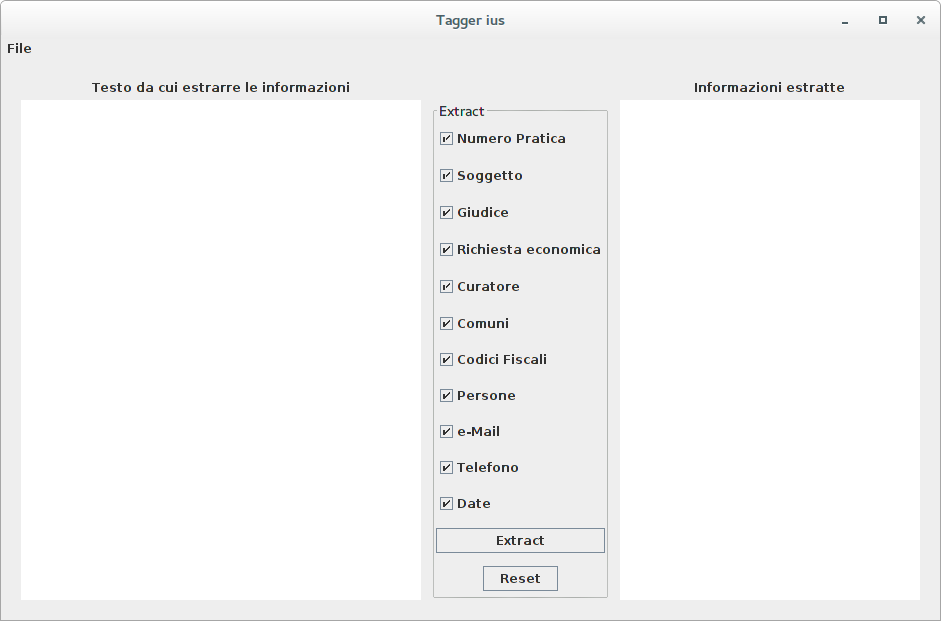
\includegraphics[width=0.8\textwidth]{img/interfaces/java-main.png}
	\caption[Schermata java main]{Schermata principale java}
	\label{java-main}
\end{figure}

Come si può vedere, l'interfaccia minimalista permette al sistema di essere facilmente usabile infatti presenta essenzialmente tre diverse sezioni ognuna dedita ad una particolare attività:
    \begin{itemize}
    	\item \textbf{Inserimento} : In questa sezione viene data la possibilità di inserire il documento testuale da cui si vogliono estrarre le informazioni; con questa operazione non si fa altro che asserire un documento da dover poi essere processato dal core prolog del sistema.
    	\item \textbf{Scelta dei tag} : In questa sezione si da la possibilità all'utente di filtrare i tag da voler estrarre dal documento attraverso la selezione/deselezione della checkbox corrispondente al tag; con questa operazione si vanno a selezionare quali saranno i tag che il core prolog deve etichettare nel documento.
    	\item \textbf{Visualizzazione} : In questa schermata invece verranno mostrate le informazioni che l'utente ha deciso di estrarre dal documento;
    	\item \textbf{Reset delle condizioni iniziali} : Tramite il pulsante \emph{Reset} si ripristineranno le condizioni iniziali del sistema. In particolare, viene ripristinato lo stato iniziale:
    	\begin{itemize}
    		\item \emph{Interfaccia} : cancellando sia le textbox contenenti il documento inserito e i tag etichettati dal testo, sia le scelte dei tag da effettuare.
    		\item \emph{Core Prolog} : ritrattando il documento appena inserito nella sezione, riportando il sistema allo stato di partenza.
    	\end{itemize}
    \end{itemize}
Inoltre è presente anche una barra di menù dalla quale viene data la possibilità di scegliere quale motore utilizzare per la comunicazione tra java e prolog tra quelli descritti in \ref{java-prolog}:
\begin{figure}[H]
	\centering
	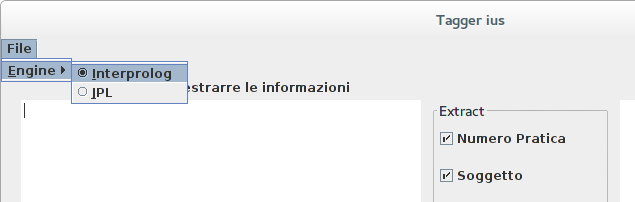
\includegraphics[width=0.9\textwidth]{img/interfaces/java-engine.png}
	\caption[Schermata java engine]{Scelta engine java - prolog}
	\label{java-engine}
\end{figure}
\clearpage
\subsubsection{Esempio di interazione}
	Supponiamo di voler taggare il seguente documento:
	
	\small
	\label{doc-example}
	\begin{Verbatim}[frame=single,framesep=3mm]
	  DOMANDA DI AMMISSIONE ALLO STATO PASSIVO
                 TRIBUNALE CIVILE DI FOGGIA
                     SEZIONE FALLIMENTARE
Procedura n. 49/2011
GIUDICE DELEGATO - Altobello Nicola
CURATORE FALLIMENTARE - Torelli Mario
                   
               DOMANDA DI AMMISSIONE AL PASSIVO

Ill.mo signor Giudice Delegato alla procedura sopra indicata, 
il sottoscritto, Rutigliano Francesco, nato a Lecce il 15 Luglio
1974, C.F. RTGFRC74L15E506K, e domiciliato a Foggia in via Roma,
12, il quale dichiara di voler ricevere comunicazioni e notifiche
al seguente n. 3475459798 oppure per email al seguente indirizzo
francesco.rutigliano@gmail.com

                            CHIEDE

di essere ammesso allo stato passivo della procedure in epigrafe
indicata:

in via chirografaria per € 1890.00
Precisando che il proprio credito deriva da prestazioni di lavoro 
subordinato in qualità di operaio.

Si allegano n. 1 documenti:
Modello prestazione occasionale

in via privilegiata per € 2000.00
Precisando che il proprio credito deriva da acquisto materiale.

Si allegano n. 3 documenti:
fattura n. 1, di € 1000;
fattura n. 2, di € 800;
fattura n. 3, di € 200.

Foggia, 15 settembre 2013

                                         Rutigliano Francesco
	\end{Verbatim}

Come mostrato nella figura sottostante, dovremo innanzitutto inserire il testo del documento nella sezione apposita:
\begin{figure}[H]
	\centering
	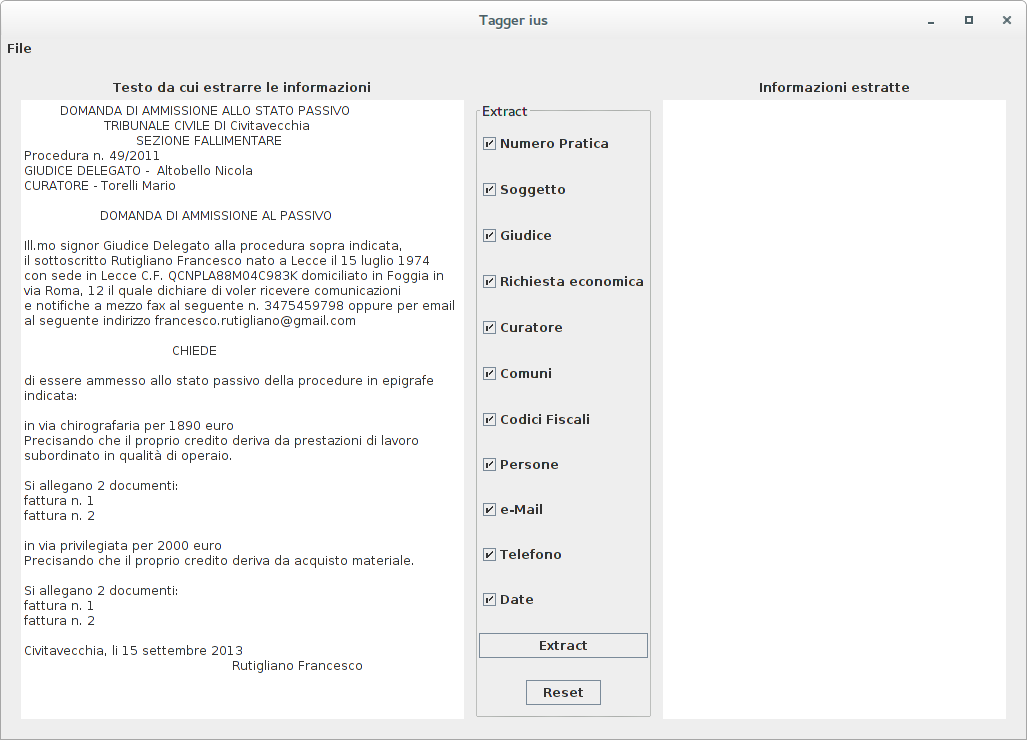
\includegraphics[width=1.1\textwidth]{img/interfaces/java-document.png}
	\caption[Schermata java document]{Inserimento testo del documento}
	\label{java-doc}
\end{figure}

Successivamente, dopo aver deciso quali tag far fare al sistema (nel nostro caso verranno selezionati tutti), si passerà all'esecuzione dell'estrazione vera e propria tramite l'apposito tasto \emph{Extract}.

In seguito all'estrazione, verranno mostrati a video tutti i tag che il sistema è riuscito ad estrarre dal testo passato come input. Di seguito un esempio di schermata di output basata sul documento definito in precedenza.

\begin{figure}[H]
	\centering
	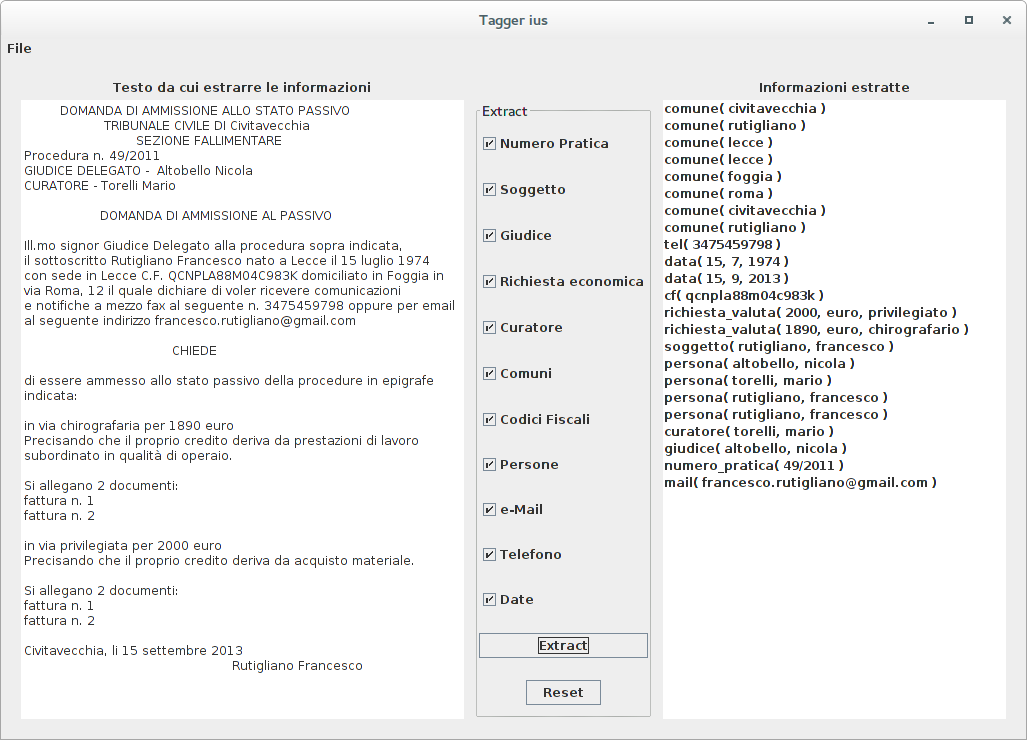
\includegraphics[width=1.1\textwidth]{img/interfaces/java-result.png}
	\caption[Schermata java result]{Risultati estrazione dei tag}
	\label{java-result}
\end{figure}

A partire da questo output, viene data la possibilità all'utente anche di capire come è stato ottenuto un particolare tag; infatti, cliccando su un tag, comparirà una nuova finestra nella quale verranno mostrati sia in maniera testuale che in maniera grafica come è stato ottenuto il tag.
Ad esempio, qualora l'utente volesse visionare il tag relativo alla richiesta valuta di 2000 euro, comparirà la seguente schermata:

\begin{figure}[H]
	\centering
	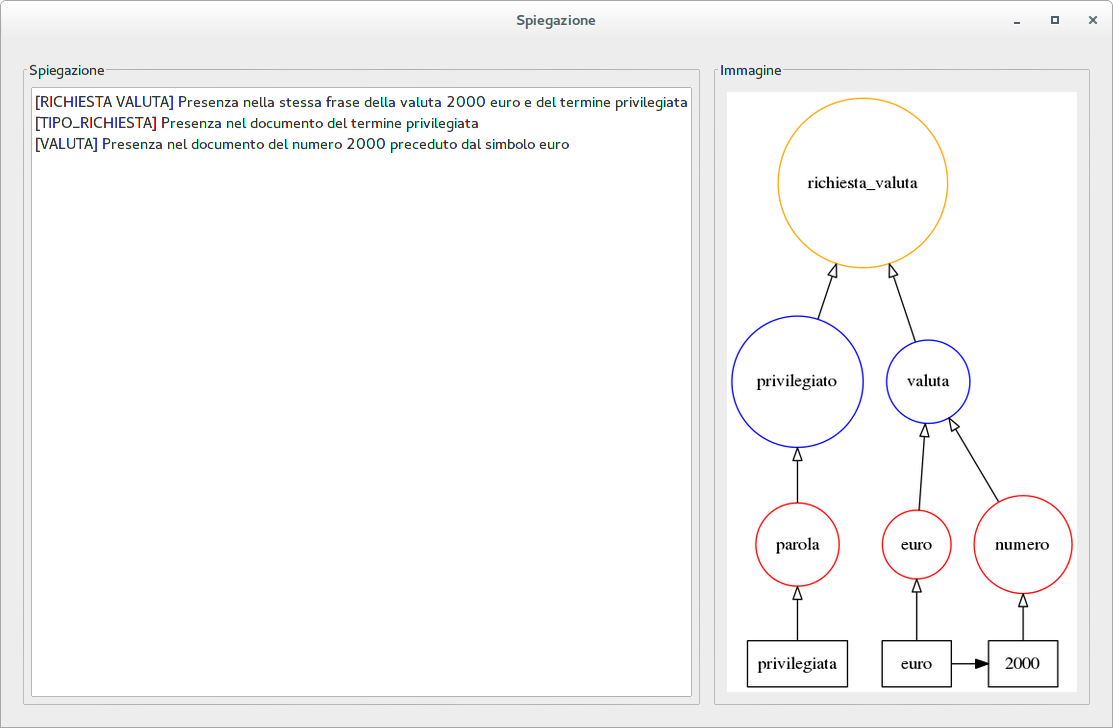
\includegraphics[width=1.1\textwidth]{img/interfaces/java-richiestavaluta.png}
	\caption[Schermata java explain richiesta valuta]{Spiegazione \emph{richiesta valuta}}
	\label{java-richiestavaluta}
\end{figure}

Un altro esempio potrebbe essere la spiegazione relativa all'individuazione del tag curatore su \emph{Mario Torelli}:

\begin{figure}[H]
	\centering
	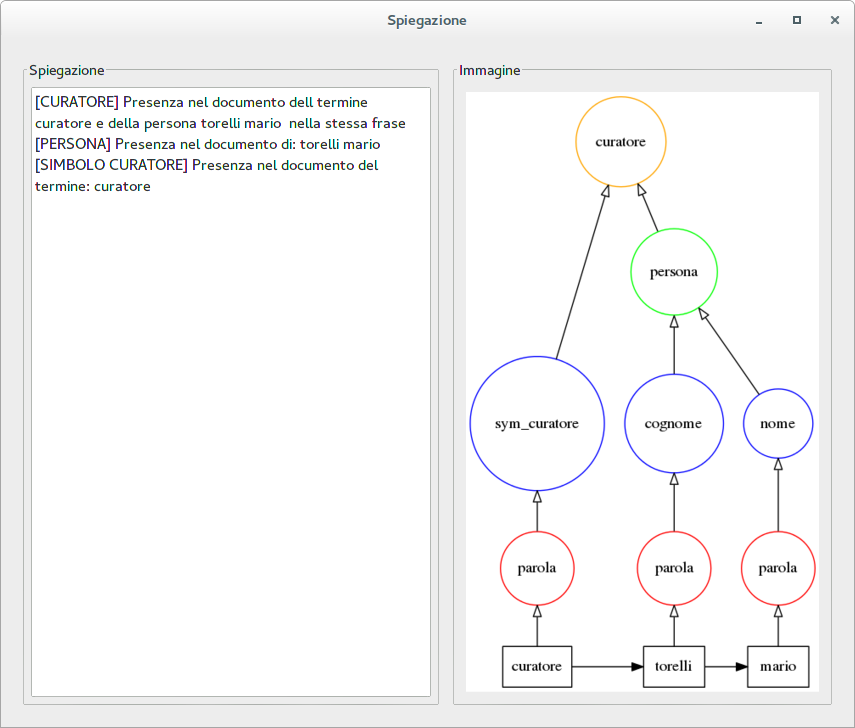
\includegraphics[width=0.8\textwidth]{img/interfaces/java-curatore.png}
	\caption[Schermata java explain curatore]{Spiegazione \emph{curatore}}
	\label{java-curatore}
\end{figure}

Infine un esempio di numero pratica potrebbe essere:

\begin{figure}[H]
	\centering
	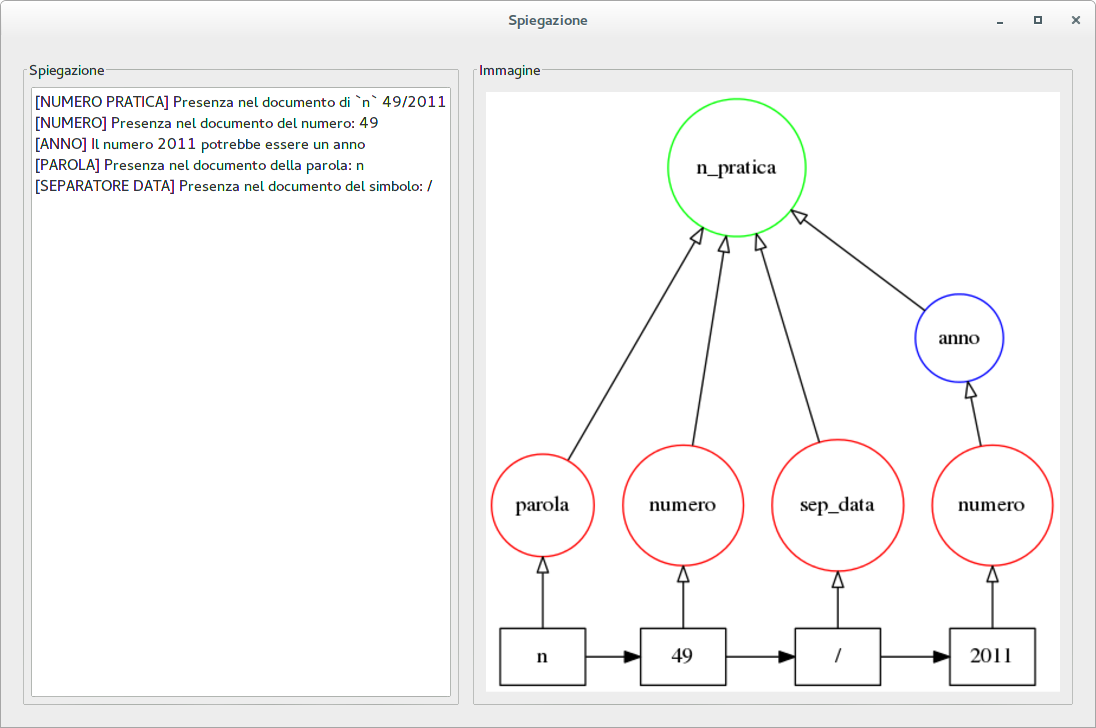
\includegraphics[width=0.8\textwidth]{img/interfaces/java-pratica.png}
	\caption[Schermata java explain numero pratica]{Spiegazione \emph{numero pratica}}
	\label{java-pratica}
\end{figure}

\subsection{Testuale}
Come detto in precedenza, l’interazione avviene principalmente tramite l'interfaccia grafica descritta nella sezione precedente ma viene data anche la possibilità di interagire con il sistema anche senza l'ausilio di tale interfaccia, utilizzando direttamente l'interprete Prolog da terminale, previa consultazione del modulo principale del sistema denominato \emph{main.pl}; le funzionalità del sistema sono indipendenti dal metodo con cui si vuole interagire con il sistema stesso. Inoltre, le funzionalità offerte sono le medesime sia per l'interfaccia grafica che per l'interfaccia testuale.

\subsubsection{Esempio di interazione}
Supponiamo di voler taggare lo stesso documento definito nella sezione precedente \ref{doc-example}; in questo caso, il sistema si presenterà all'utente tramite la seguente schermata:

\begin{figure}[H]
	\centering
	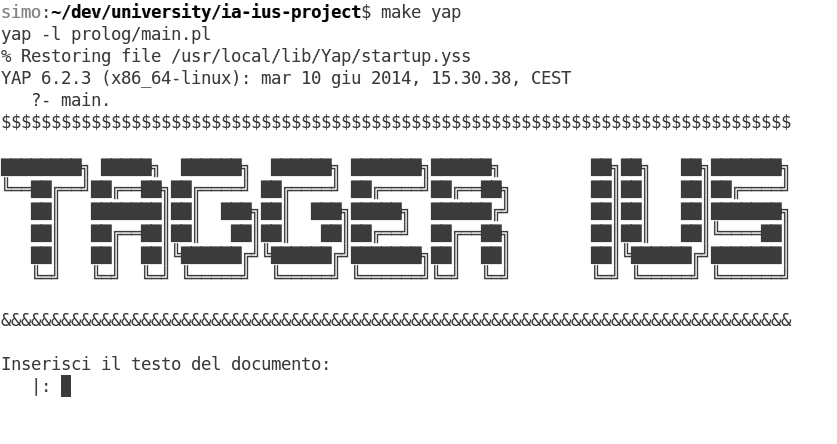
\includegraphics[width=0.9\textwidth]{img/interfaces/CLI-main.png}
	\caption[Schermata CLI main]{Schermata principale CLI}
	\label{CLI-main}
\end{figure}

Anche in questo caso, è richiesto l'inserimento del testo del documento da taggare, ma a differenza dell'input da dare al sistema java, in questo caso bisognerà far precedere e succedere il testo da delle virgolette.
Inoltre, ogni input dovrà necessariamente terminare con un punto fermo.

\begin{figure}[H]
	\centering
	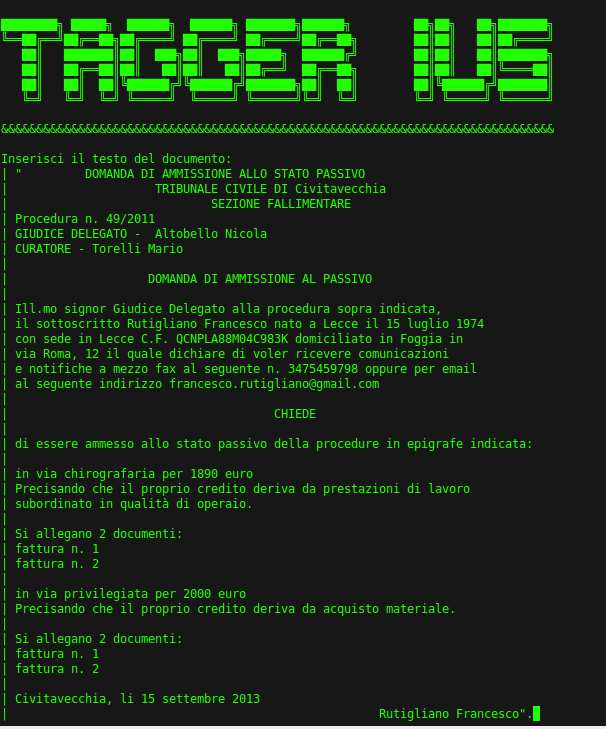
\includegraphics[width=0.9\textwidth]{img/interfaces/CLI-document.png}
	\caption[Schermata CLI document]{Inserimento testo del documento}
	\label{CLI-doc}
\end{figure}

Una volta inserito il testo da analizzare, il sistema darà la possibilità all'utente di selezionare quali tag estrarre attraverso l'ausilio di un menù testuale a scelta numerica.

\begin{figure}[H]
	\centering
	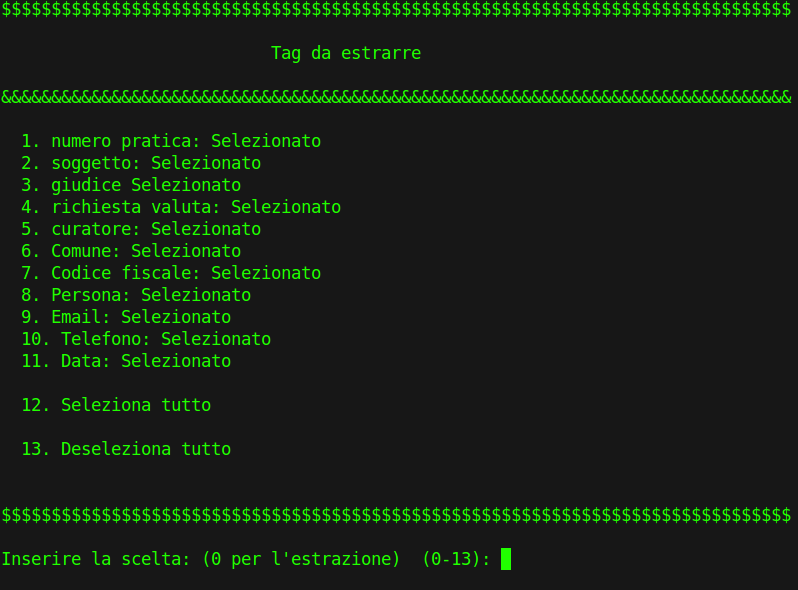
\includegraphics[width=0.9\textwidth]{img/interfaces/CLI-tagSelect.png}
	\caption[Schermata CLI tag select]{Menù di selezione dei tag}
	\label{CLI-tagSelect}
\end{figure}

Terminata la configurazione del sistema definendo quali tag analizzare, il sistema procederà all'elaborazione del testo; L'output del sistema sarà di questo tipo:
\begin{figure}[H]
	\centering
	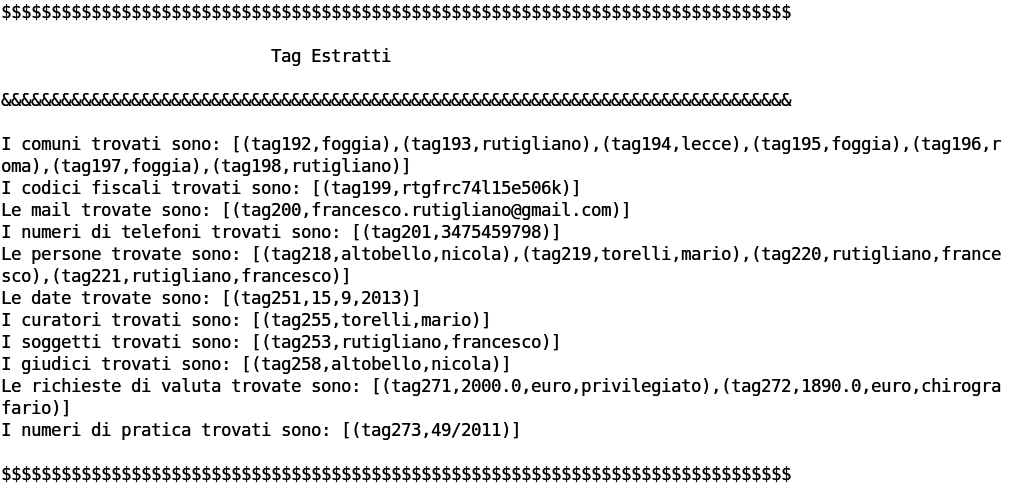
\includegraphics[width=0.9\textwidth]{img/interfaces/CLI-result.png}
	\caption[Schermata CLI result]{Risultati estrazione dei tag}
	\label{CLI-result}
\end{figure}

Come si può vedere, ogni risultato estratto avrà un tag identificativo necessario al fine di poter ottenere la spiegazione di come è stato ottenuto quel tag. In particolare, il sistema chiederà all'utente se vuole verificare come è stato ottenuto qualche particolare tag; qualora l'utente volesse, ad esempio verificare come è stata ottenuta la richiesta valuta di tipo privilegiata di 2000 euro, dovrà inserire il corrispettivo tag identificativo, in questo caso \emph{tag271}:

\begin{figure}[H]
	\centering
	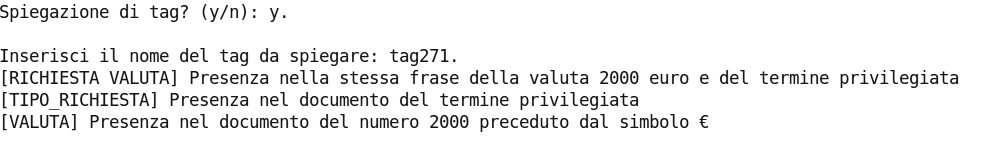
\includegraphics[width=0.9\textwidth]{img/interfaces/CLI-spiegazioneRich.png}
	\caption[Schermata CLI spiegazione]{Spiegazione tag \emph{richiesta valuta}}
	\label{CLI-spiegaRichiesta}
\end{figure}

Di seguito altri esempi di spiegazione, in particolare di come è stato riconosciuto un \emph{curatore} e un \emph{numero di pratica}:
\begin{figure}[H]
	\centering
	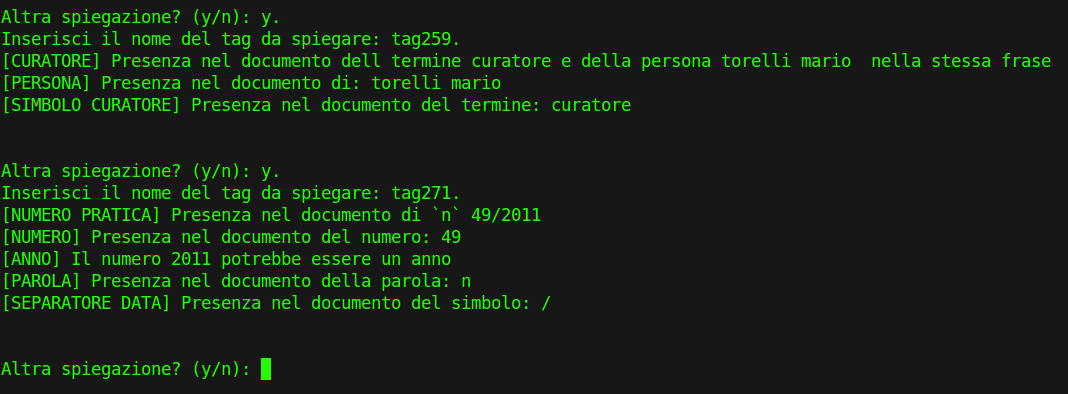
\includegraphics[width=0.9\textwidth]{img/interfaces/CLI-spiegazione.png}
	\caption[Schermata CLI altre spiegazioni]{Spiegazione tag \emph{curatore} e \emph{numero pratica}}
	\label{CLI-spiega}
\end{figure}